\subsection{Amplificatore differenziale}

\begin{figure}[h]
    \centering
    \begin{minipage}{0.49\textwidth}
        \centering
        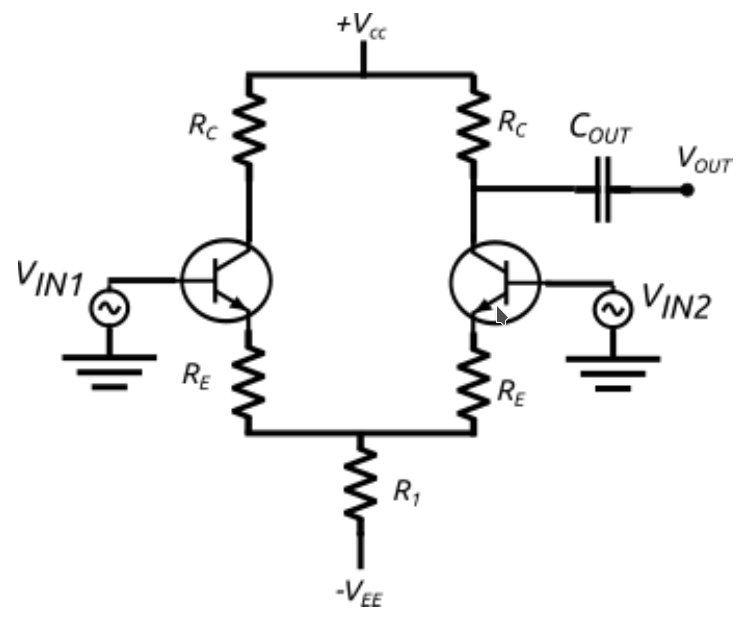
\includegraphics[width=\textwidth]{amp_diff_circ.png} 
        \caption{Amplificatore differenziale senza gene\-ratore corrente costante}
        \label{fig:ampdiff_circ}
    \end{minipage}\hfill
    \begin{minipage}{0.49\textwidth}
        \centering
        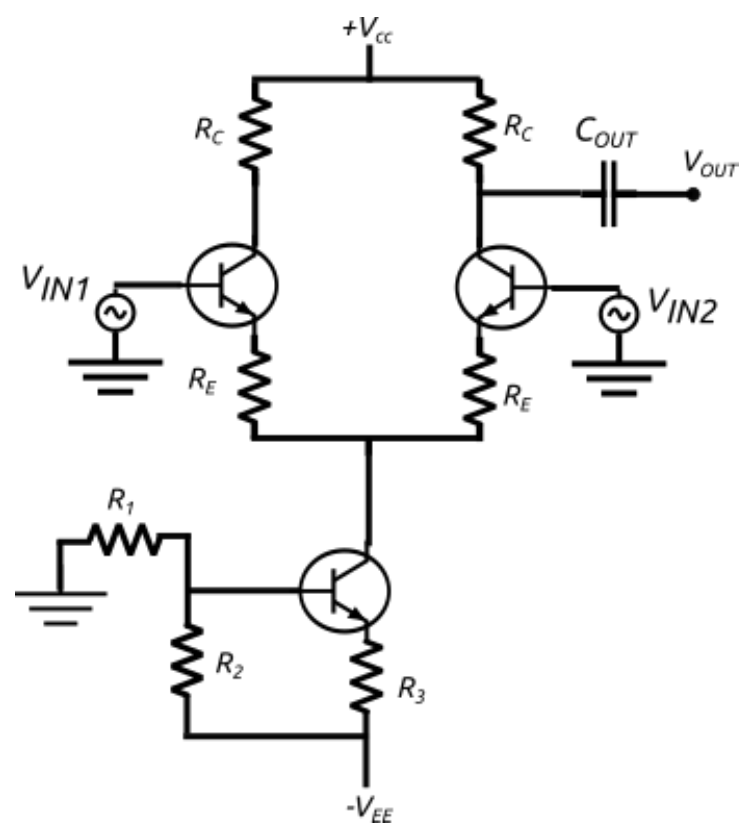
\includegraphics[width=\textwidth]{amp_diff_cc_circ.png} 
        \caption{Amplificatore differenziale con gene\-ratore corrente costante}
        \label{fig:ampdiff_cc_circ}
    \end{minipage}
\end{figure}

Vengono ora mostrati i risultati dei guadagni nelle diverse configurazioni e gli eventuali confronti \ref{fig:gains}.

\begin{figure}[h]
    \centering
    \begin{minipage}{0.5\textwidth}
        \centering
        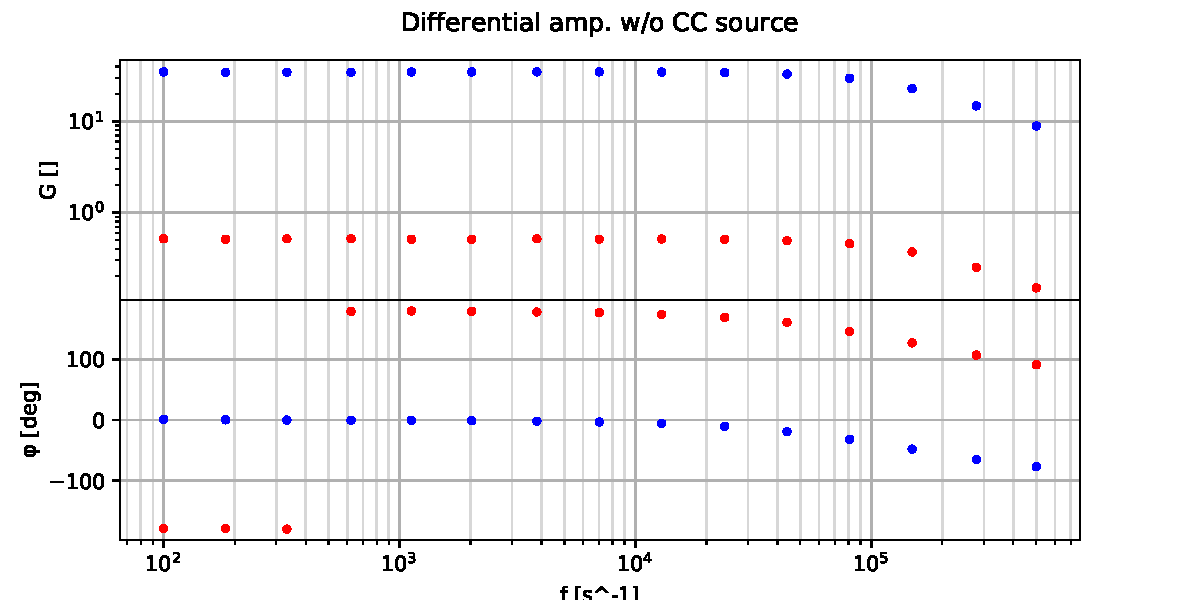
\includegraphics[width=\textwidth]{Figure_1.pdf} 
        %\caption{first figure}
    \end{minipage}\hfill
    \begin{minipage}{0.5\textwidth}
        \centering
        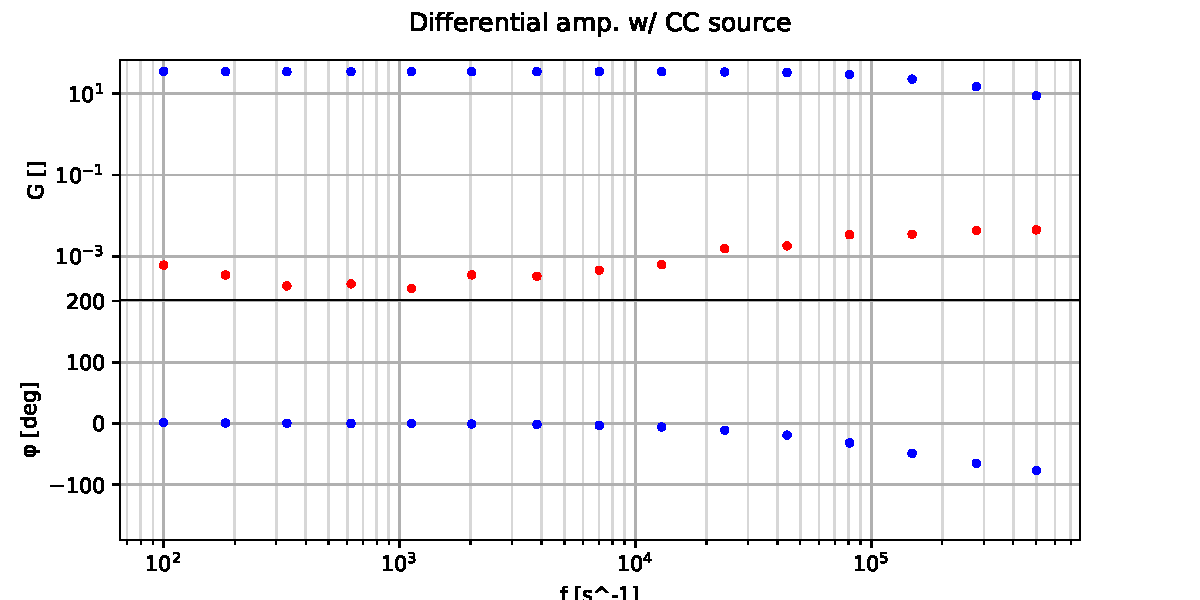
\includegraphics[width=\textwidth]{Figure_2.pdf} 
        %\caption{second figure}
    \end{minipage}
    \\
    \centering
    \begin{minipage}{0.5\textwidth}
        \centering
        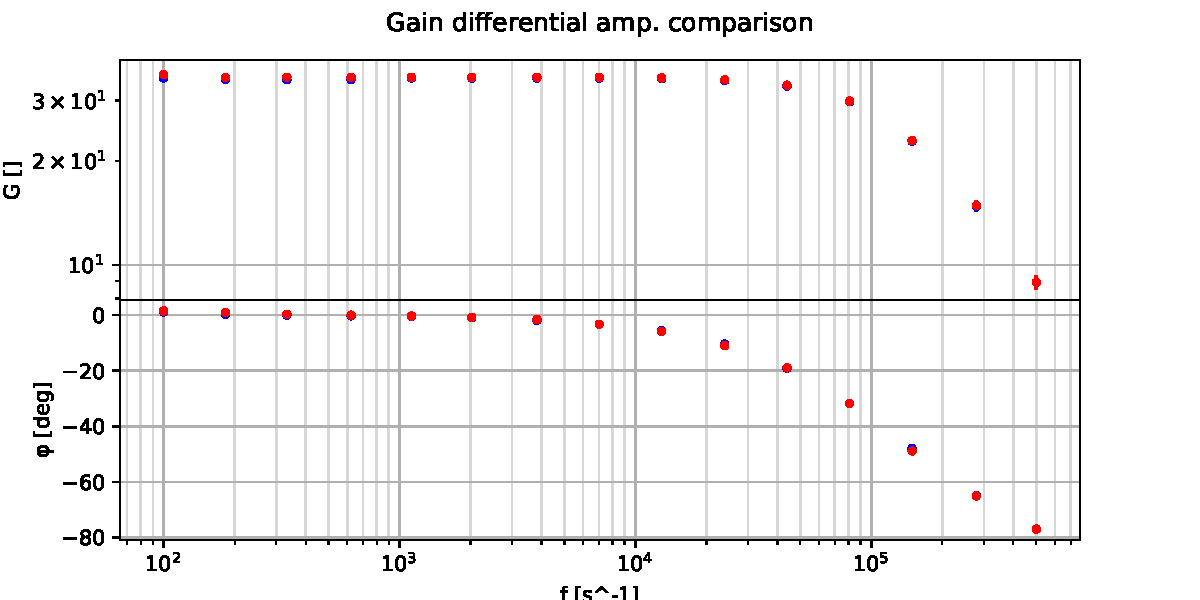
\includegraphics[width=\textwidth]{Figure_3.pdf} 
        %\caption{first figure}
    \end{minipage}\hfill
    \begin{minipage}{0.5\textwidth}
        \centering
        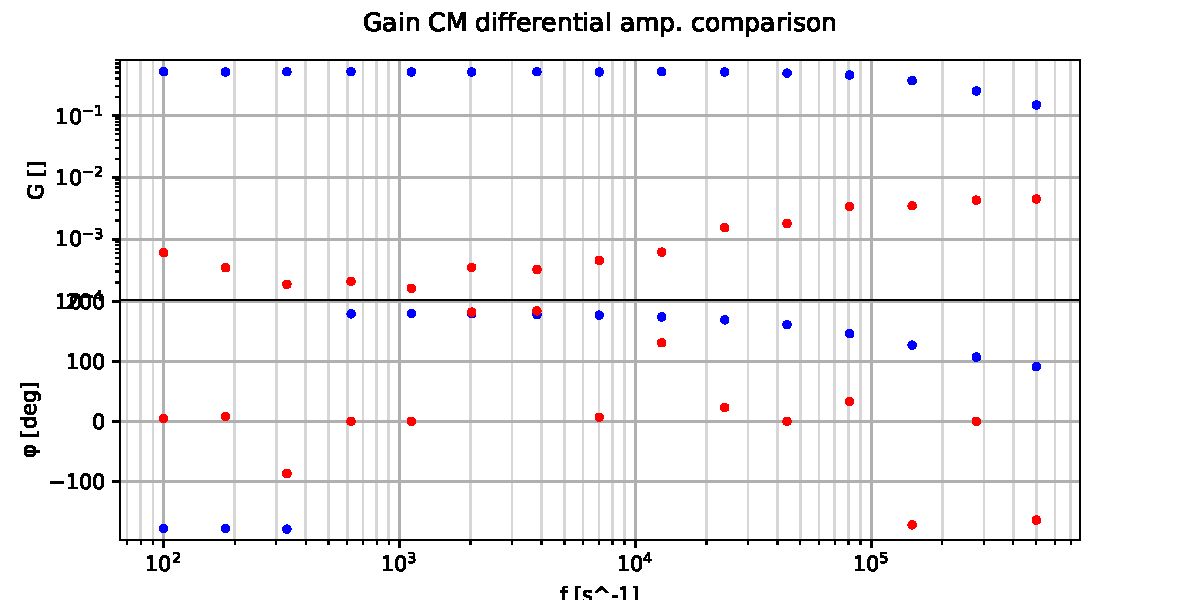
\includegraphics[width=\textwidth]{Figure_4.pdf} 
        %\caption{second figure}
    \end{minipage}
    \caption{Grafici di Bode dei guadagni, spiegazione nel testo.}
    \label{fig:gains}
\end{figure}

Nella riga in alto sono mostrati i guadagni differenziale (in blu) e modo comune (in rosso), senza e con il generatore di corrente costante. Notare innanzitutto che nel diagramma di fase a sinistra il guadagno modo comune passa da $-180 \si{\deg}$ a $+180 \si{\deg}$ per ciclicit\'a degli angoli. Inoltre la fase modo comune con il generatore di corrente non \'e stata misurata per impossibilit\'a di una definizione di essa dato il rumore.\\
Nella riga inferiore sono mostrati i miglioramenti che si ottengono separatamente per i due tipi di guadagno nel caso con (in rosso) e senza (in blu) generatore di corrente costante, come ci aspettiamo il guadagno $G_{diff}$ non risente della circuiteria in pi\'u mentre il modo comune migliora (quindi diminuisce) considerevolmente.\\

Si procede quindi al confronto con un modello di alcune quantit\'a. \\
Il guadagno $G_{diff}$ pu\'o essere calcolato in modo pi\'u preciso con la formula:
\begin{gather}
	G_{diff}=\frac{R_C}{2*(R_E+r_e(i_0))}
\end{gather}
Quindi sapendo che $G_{diff\ max}=35.65$ si pu\'o ottenere il valore di $r_e$:
\begin{gather}
	r_e(i_0)=\frac{R_C-2 G_{diff} R_E}{2 G_{diff}}=40\si{\ohm}
\end{gather}
la quale \'e in linea con quello che ci aspetteremmo per la resistenza di emettitore di un BJT data la corrente $i_0$.

L'impedenza in parallelo al generatore di corrente $Z_S$ pu\'o essere estratta dai dati secondo:
\begin{gather}
	G_{CM}=-\frac{Z_S}{2 R_S} \\
	Z_S(\omega) = -\frac{R_C}{2 G_{CM}}
\end{gather}
e risulta avere un andamento in funzione della frequenza mostrata in figura \ref{fig:zs}.
\begin{figure}[h]
	\centering
    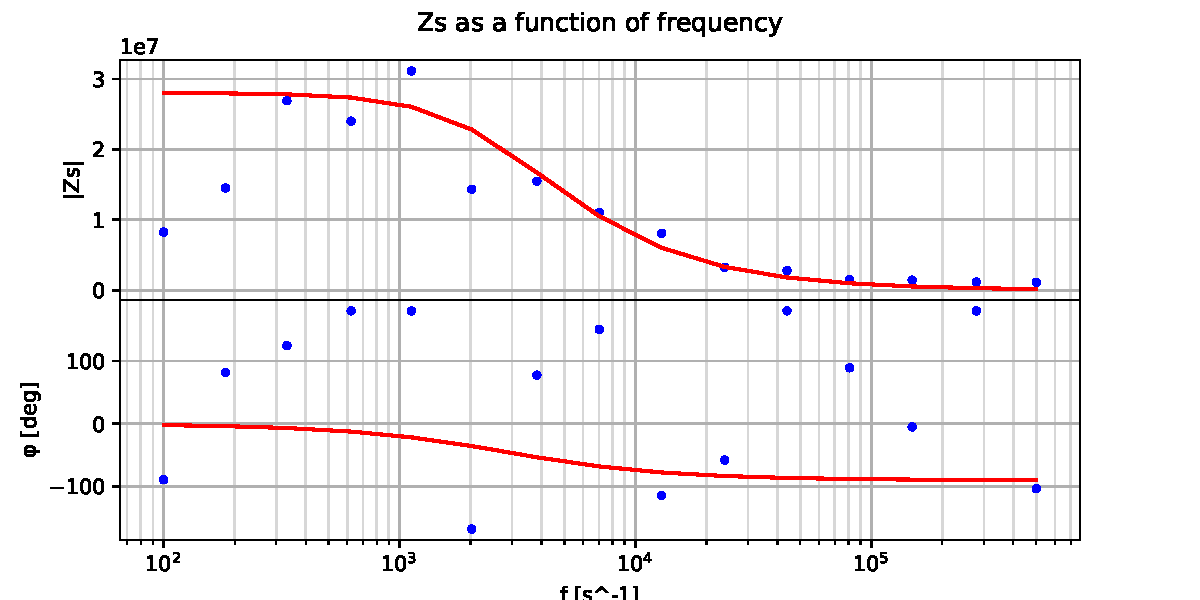
\includegraphics[width=\textwidth]{Figure_5.pdf}
    \label{fig:zs}
    \caption{Andamento di $Z_S$ in funzione della frequenza.}
\end{figure}
Nuovamente la fase misurata di $Z_S$ non \'e affidabile per via del rumore nella misurazione della fase di $G_{CM}$, tuttavia il modulo (in blu) segue l'andamento aspettato superati i $30\si{\kilo\hertz}$ scendendo a $0\si{\ohm}$ il quale \'e compatibile con l'impedenza di un condensatore da $2\si{\pico\farad}$ in parallelo ad una resistenza da $28\si{\mega\ohm}$ mostrati in rosso nella figura entrambi nel range di valori che caratterizzano la giunzione PN del transistor.

\begin{figure}[h]
    \begin{center}
    \begin{circuitikz} []
    \draw
        (0,2) to [sV,l_=$V_{IN} G_{diff}$] (0,0)
        (0,0) to (5,0)
        (0,2) to [R,l=$R_C$] (2,2) 
        (2,2) to [C,l=$C_{out}$] (3,2)
        (3,2) to [C,l_=$C_{osc}$] (3,0)
        (4,2) to [R,l=$R_{osc}$] (4,0)
        (2,2) to (5,2)
        (5,2) to [open, *-*] (5,0);
    \end{circuitikz}
    \caption{Modello $G_{diff}$ misurata.}
    \label{fig:Gdiffmodel}
    \end{center}
\end{figure}

La funzione di trasferimento per il guadagno differenziale tenuto conto del circuito di misura misurato \ref{fig:Gdiffmodel} \'e:
\begin{gather}
	H=G_{diff} \frac{R_{osc} \pars \frac{1}{j\omega C_{osc}}}{R_{osc} \pars \frac{1}{j\omega C_{osc}} + \frac{1}{j\omega C_{out}} + R_C}
\end{gather}
la quale pu\'o essere confrontata, ponendo i valori ottenuti nelle precedenti esperienze per $C_{osc}=110\si{\pico\farad}$ $R_{osc}=1\si{\mega\ohm}$ e il condensatore $C_{out}=100\si{\nano\farad}$ posto in uscita con i dati sperimentali ottenuti in figura \ref{fig:gain_model}.

\begin{figure}[h]
	\centering
    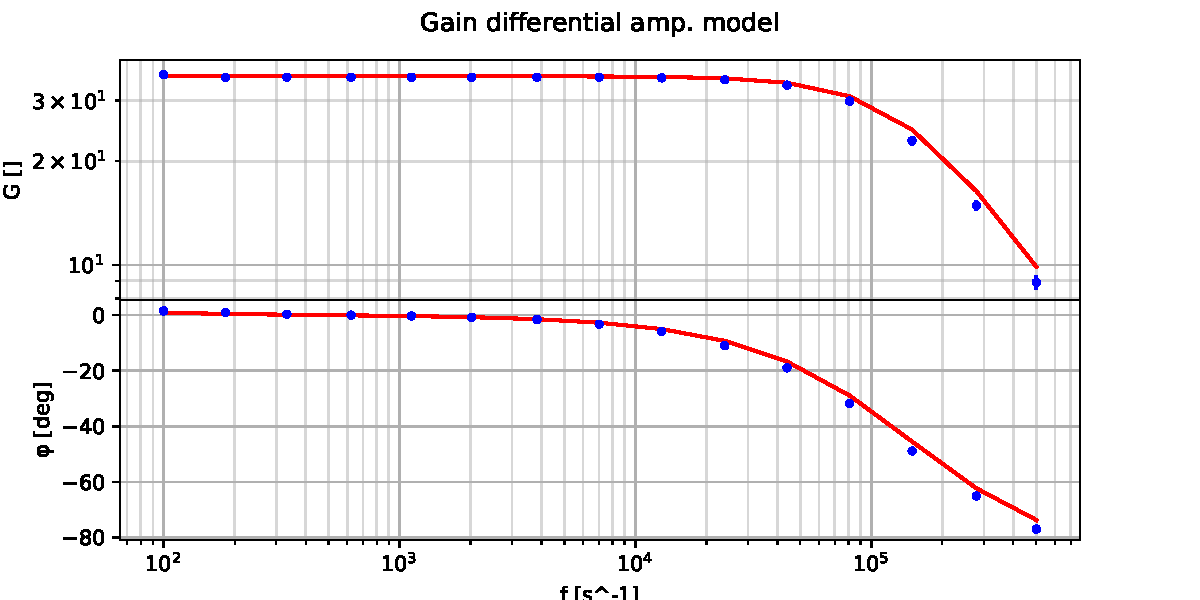
\includegraphics[width=\textwidth]{Figure_6.pdf}
    \label{fig:gain_model}
    \caption{Gain in funzione della frequenza, in blu i punti sperimentali e in rosso la curva del modello.}
\end{figure}
 
 